% answers.tex —— 2008 年·普通高等学校招生考试·江苏卷 · 参考答案与详细解析片段
% 由 tools/generate_projects.py 依来源总账自 2008/2008_数学真题_江苏_试题.md + 2008/2008_数学真题_江苏_解析正文.md + 2008/2008_数学真题_江苏_答案要点.md 生成，勿手改（改源 MD 后重跑）


\begin{gktip}
固定候选 PDF 仅含题面、无答案与解析；以下为非官方编者独立推导。
\end{gktip}

\begin{answer}
\gksolhead{1}{}

\textbf{题目}：

若函数 $f(x)=\cos\left(\omega x-\dfrac{\pi}6\right)$（$\omega>0$）最小正周期为 $\dfrac{\pi}5$，则 $\omega=$\gkblank{}。

\Needspace{4\baselineskip}
\textbf{解析}

$T=\dfrac{2\pi}\omega=\dfrac{\pi}5$，故 $\omega=10$。

\gkanswer{答案：$10$。}

\end{answer}
\begin{answer}
\gksolhead{2}{}

\textbf{题目}：

若将一颗质地均匀的骰子（一种各面上分别标有 $1$，$2$，$3$，$4$，$5$，$6$ 个点的正方体玩具）先后抛掷 $2$ 次，则出现向上的点数之和为 $4$ 的概率是\gkblank{}。

\Needspace{4\baselineskip}
\textbf{解析}

点数和为 $4$ 的情形为 $(1,3)$、$(2,2)$、$(3,1)$ 共 $3$ 种，故 $P=\dfrac3{36}=\dfrac1{12}$。

\gkanswer{答案：$\dfrac1{12}$。}

\end{answer}
\begin{answer}
\gksolhead{3}{}

\textbf{题目}：

若将复数 $\dfrac{1+\mathrm i}{1-\mathrm i}$ 表示为 $a+b\mathrm i$（$a$，$b\in\mathbf R$，$\mathrm i$ 是虚数单位）的形式，则 $a+b=$\gkblank{}。

\Needspace{4\baselineskip}
\textbf{解析}

$\dfrac{1+\mathrm i}{1-\mathrm i}=\dfrac{(1+\mathrm i)^2}2=\mathrm i$，故 $a=0$，$b=1$，$a+b=1$。

\gkanswer{答案：$1$。}

\end{answer}
\begin{answer}
\gksolhead{4}{}

\textbf{题目}：

设集合 $A=\left\{x\mid (x-1)^2<3x+7,\ x\in\mathbf R\right\}$，则集合 $A\cap\mathbf Z$ 中有\gkblank{}个元素。

\Needspace{4\baselineskip}
\textbf{解析}

$(x-1)^2<3x+7\iff x^2-5x-6<0\iff-1<x<6$，其中整数为 $0,1,2,3,4,5$，共 $6$ 个。

\gkanswer{答案：$6$。}

\end{answer}
\begin{answer}
\gksolhead{5}{}

\textbf{题目}：

已知向量 $\boldsymbol a$ 与 $\boldsymbol b$ 的夹角为 $120^\circ$，$|\boldsymbol a|=1$，$|\boldsymbol b|=3$，则 $|5\boldsymbol a-\boldsymbol b|=$\gkblank{}。

\Needspace{4\baselineskip}
\textbf{解析}

\Needspace{5\baselineskip}
$\boldsymbol a\cdot\boldsymbol b=1\times3\times\left(-\dfrac12\right)=-\dfrac32$，故

\nopagebreak[4]
\[|5\boldsymbol a-\boldsymbol b|^2=25|\boldsymbol a|^2-10\boldsymbol a\cdot\boldsymbol b+|\boldsymbol b|^2=25+15+9=49.\]

\gkanswer{答案：$7$。}

\end{answer}
\begin{answer}
\gksolhead{6}{}

\textbf{题目}：

在平面直角坐标系 $xOy$ 中，设 $D$ 是横坐标与纵坐标的绝对值均不大于 $2$ 的点构成的区域，$E$ 是到原点的距离不大于 $1$ 的点构成的区域。向 $D$ 中随机投一点，则所投的点落在 $E$ 中的概率是\gkblank{}。

\Needspace{4\baselineskip}
\textbf{解析}

$D$ 是边长为 $4$ 的正方形（面积 $16$），$E$ 是单位圆（面积 $\pi$），故 $P=\dfrac{\pi}{16}$。

\gkanswer{答案：$\dfrac{\pi}{16}$。}

\end{answer}
\begin{answer}
\gksolhead{7}{}

\textbf{题目}：

某地区为了解 $70\sim80$ 岁老人的日平均睡眠时间（单位：h），随机选择了 $50$ 位老人进行调查。下表是 $50$ 位老人日睡眠时间频率分布表：

\begin{center}
\begin{tabular}{lllll}
\toprule
序号（$i$） & 分组（睡眠时间） & 组中值（$G_i$） & 频数（人数） & 频率（$F_i$） \\
\midrule
$1$ & $[4,5)$ & $4.5$ & $6$ & $0.12$ \\
$2$ & $[5,6)$ & $5.5$ & $10$ & $0.20$ \\
$3$ & $[6,7)$ & $6.5$ & $20$ & $0.40$ \\
$4$ & $[7,8)$ & $7.5$ & $10$ & $0.20$ \\
$5$ & $[8,9)$ & $8.5$ & $4$ & $0.08$ \\
\bottomrule
\end{tabular}
\end{center}

在上述统计数据的分析中，一部分计算见算法流程图，则输出的 $S$ 的值是\gkblank{}。
\nopagebreak[4]
\begin{center}% 2008 年江苏卷第 7 题：加权平均的算法流程图。
% 来源 PDF：gaokaomath-src/普通高考/2008/2008江苏.pdf
% SHA-256：b998b93963143559a1ce800a6d320de618883b0e22ee5130b7666a2374caeba0
% 原页：2008江苏.pdf 第 1 页（A3 三栏）第 1 栏，书页码 457。
% 绘制依据：按原页流程：开始 → S←0 → i←1 → 输入 G_i,F_i → S←S+G_iF_i → 判断 i≥5 →
%   N 时 i←i+1 回到输入 → Y 时输出 S → 结束。
\begin{tikzpicture}[node distance=0.55cm, semithick, every node/.style={inner sep=3pt},
  box/.style={draw, rounded corners=1pt, minimum width=2.2cm, minimum height=0.55cm},
  io/.style={draw, trapezium, trapezium left angle=70, trapezium right angle=110,
             minimum width=2.4cm, minimum height=0.55cm},
  dec/.style={draw, diamond, aspect=2, inner sep=1pt}]

  \node[box] (start) {开始};
  \node[box, below=of start] (s0) {$S\leftarrow0$};
  \node[box, below=of s0] (i1) {$i\leftarrow1$};
  \node[io, below=of i1] (input) {输入 $G_i,F_i$};
  \node[box, below=of input] (acc) {$S\leftarrow S+G_iF_i$};
  \node[dec, below=0.5cm of acc, minimum width=1.6cm, minimum height=0.85cm] (test) {$i\geqslant5$};
  \node[io, below=0.75cm of test] (out) {输出 $S$};
  \node[box, below=of out] (end) {结束};
  \node[box, right=1.6cm of acc] (inc) {$i\leftarrow i+1$};

  \draw[->,>=stealth] (start) -- (s0);
  \draw[->,>=stealth] (s0) -- (i1);
  \draw[->,>=stealth] (i1) -- (input);
  \draw[->,>=stealth] (input) -- (acc);
  \draw[->,>=stealth] (acc) -- (test);
  \draw[->,>=stealth] (test) -- node[left] {Y} (out);
  \draw[->,>=stealth] (out) -- (end);
  \draw[->,>=stealth] (test.east) -- node[above] {N} (inc.west);
  \draw[->,>=stealth] (inc.north) |- (input.east);
\end{tikzpicture}
\end{center}
\nopagebreak[4]
\Needspace{4\baselineskip}
\textbf{解析}

\Needspace{5\baselineskip}
流程图计算 $S=\sum G_iF_i$：

\nopagebreak[4]
\[S=4.5\times0.12+5.5\times0.20+6.5\times0.40+7.5\times0.20+8.5\times0.08=6.42.\]

\gkanswer{答案：$6.42$。}

\end{answer}
\begin{answer}
\gksolhead{8}{}

\textbf{题目}：

设直线 $y=\dfrac12x+b$ 是曲线 $y=\ln x$（$x>0$）的一条切线，则实数 $b$ 的值为\gkblank{}。

\Needspace{4\baselineskip}
\textbf{解析}

设切点横坐标为 $x_0$，由 $\dfrac1{x_0}=\dfrac12$ 得 $x_0=2$，切点 $(2,\ln2)$。代入 $y=\dfrac12x+b$ 得 $\ln2=1+b$，故 $b=\ln2-1$。

\gkanswer{答案：$\ln2-1$。}

\end{answer}
\begin{answer}
\gksolhead{9}{}

\textbf{题目}：

如图，在平面直角坐标系 $xOy$ 中，设三角形 $ABC$ 的顶点分别为 $A(0,a)$，$B(b,0)$，$C(c,0)$；点 $P(0,p)$ 为线段 $AO$ 上的一点（异于端点），这里 $a$，$b$，$c$，$p$ 为非零实数。设直线 $BP$，$CP$ 分别与边 $AC$，$AB$ 交于点 $E$，$F$。某同学已正确求得 $OE$ 的方程：$\left(\dfrac1b-\dfrac1c\right)x+\left(\dfrac1p-\dfrac1a\right)y=0$。请你完成直线 $OF$ 的方程：$\left(\rule{3em}{0.4pt}\right)x+\left(\dfrac1p-\dfrac1a\right)y=0$。

\Needspace{4\baselineskip}
\textbf{解析}

$OE$ 的方程形如 $\left(\dfrac1b-\dfrac1c\right)x+\left(\dfrac1p-\dfrac1a\right)y=0$（其中 $b$ 对应点 $B$、$c$ 对应点 $C$）；$OF$ 与 $OE$ 关于 $A$、$O$ 的地位对称，$b$、$c$ 互换，故填 $\dfrac1c-\dfrac1b$。

\gkanswer{答案：$\dfrac1c-\dfrac1b$。}

\end{answer}
\begin{answer}
\gksolhead{10}{}

\textbf{题目}：

\Needspace{5\baselineskip}
将全体正整数排成一个三角形数阵：

\nopagebreak[4]
\[\begin{array}{cccccc}&&1&&&\\&&2&3&&\\&4&5&6&&\\7&8&9&10&&\\\cdots&\cdots&\cdots&\cdots&&\end{array}\]

根据以上排列规律，数阵中第 $n$（$n\geqslant3$）行的从左向右的第 $3$ 个数是\gkblank{}。

\Needspace{4\baselineskip}
\textbf{解析}

第 $n-1$ 行最后一个数为 $\dfrac{(n-1)n}2$，故第 $n$ 行第 $3$ 个数为 $\dfrac{(n-1)n}2+3$。

\gkanswer{答案：$\dfrac{(n-1)n}2+3$。}

\end{answer}
\begin{answer}
\gksolhead{11}{}

\textbf{题目}：

设 $x$，$y$，$z$ 为正实数，满足 $x-2y+3z=0$，则 $\dfrac{y^2}{xz}$ 的最小值为\gkblank{}。

\Needspace{4\baselineskip}
\textbf{解析}

\Needspace{5\baselineskip}
由 $x-2y+3z=0$ 得 $y=\dfrac{x+3z}2$，故

\nopagebreak[4]
\[\frac{y^2}{xz}=\frac{x^2+6xz+9z^2}{4xz}=\frac14\left(\frac xz+\frac{9z}x+6\right)\geqslant\frac14(6+6)=3,\]

当 $x=3z$ 时取等号。

\gkanswer{答案：$3$。}

\end{answer}
\begin{answer}
\gksolhead{12}{}

\textbf{题目}：

在平面直角坐标系 $xOy$ 中，设椭圆 $\dfrac{x^2}{a^2}+\dfrac{y^2}{b^2}=1$（$a>b>0$）的焦距为 $2c$，以点 $O$ 为圆心、$a$ 为半径作圆 $M$。若过点 $\left(\dfrac{a^2}{c},0\right)$ 所作圆 $M$ 的两条切线互相垂直，则该椭圆的离心率 $e=$\gkblank{}。

\Needspace{4\baselineskip}
\textbf{解析}

过 $P\left(\dfrac{a^2}c,0\right)$ 的两条切线互相垂直等价于 $|OP|=a\sqrt2$，即 $\dfrac{a^2}c=a\sqrt2$，故 $a=\sqrt2c$，$e=\dfrac ca=\dfrac{\sqrt2}2$。

\gkanswer{答案：$\dfrac{\sqrt2}2$。}

\end{answer}
\begin{answer}
\gksolhead{13}{}

\textbf{题目}：

满足条件 $AB=2$，$AC=\sqrt2BC$ 的三角形 $ABC$ 的面积的最大值是\gkblank{}。

\Needspace{4\baselineskip}
\textbf{解析}

\Needspace{5\baselineskip}
设 $BC=t$，则 $AC=\sqrt2t$，面积 $S=\dfrac12\cdot2\cdot\sqrt2t\sin A=\sqrt2t\sin A$。由余弦定理

\nopagebreak[4]
\[\cos A=\frac{4+2t^2-t^2}{4\sqrt2t}=\frac{t^2+4}{4\sqrt2t},\]

\Needspace{5\baselineskip}
于是

\nopagebreak[4]
\[S^2=2t^2\left[1-\frac{(t^2+4)^2}{32t^2}\right]=2t^2-\frac{(t^2+4)^2}{16}.\]

令 $u=t^2$，$S^2=2u-\dfrac{(u+4)^2}{16}$ 在 $u=12$ 处取最大值 $8$，此时 $\cos A=\dfrac{16}{8\sqrt6}<1$ 合法，故 $S_{\max}=2\sqrt2$。

\gkanswer{答案：$2\sqrt2$。}

\end{answer}
\begin{answer}
\gksolhead{14}{}

\textbf{题目}：

设函数 $f(x)=ax^3-3x+1$（$x\in\mathbf R$），若对于任意 $x\in[-1,1]$，都有 $f(x)\geqslant0$ 成立，则实数 $a$ 的值为\gkblank{}。

\Needspace{4\baselineskip}
\textbf{解析}

$x=0$ 时 $f(0)=1>0$。当 $x\in(0,1]$ 时，$f(x)\geqslant0\iff a\geqslant\dfrac{3x-1}{x^3}$；当 $x\in[-1,0)$ 时，$f(x)\geqslant0\iff a\leqslant\dfrac{3x-1}{x^3}$。记 $g(x)=\dfrac{3x-1}{x^3}$，$g'(x)=\dfrac{3-6x}{x^4}$，故 $g$ 在 $(0,1]$ 上的最大值为 $g\left(\dfrac12\right)=4$，在 $[-1,0)$ 上的最小值为 $g(-1)=4$。于是 $a\geqslant4$ 且 $a\leqslant4$，即 $a=4$（此时 $f(x)=(2x-1)^2(x+1)\geqslant0$）。

\gkanswer{答案：$4$。}

\end{answer}
\begin{answer}
\gksolhead{15}{}

\textbf{题目}：

如图，在平面直角坐标系 $xOy$ 中，以 $Ox$ 轴为始边做两个锐角 $\alpha$，$\beta$，它们的终边分别与单位圆交于 $A$、$B$ 两点。已知 $A$、$B$ 的横坐标分别为 $\dfrac{\sqrt2}{10}$，$\dfrac{2\sqrt5}5$。

（1）求 $\tan(\alpha+\beta)$ 的值；

（2）求 $\alpha+2\beta$ 的值。
\nopagebreak[4]
\begin{center}% 2008 年江苏卷第 15 题：单位圆上两点 A、B，终边与 Ox 轴成锐角 α、β。
% 来源 PDF：gaokaomath-src/普通高考/2008/2008江苏.pdf
% SHA-256：b998b93963143559a1ce800a6d320de618883b0e22ee5130b7666a2374caeba0
% 原页：2008江苏.pdf 第 1 页（A3 三栏）第 2 栏，书页码 457。
% 绘制依据：按原页画单位圆、x/y 轴、O，A 在第一象限靠近 y 轴、B 在第一象限靠近 x 轴，
%   α、β 分别标在 OA、OB 与 x 轴之间。
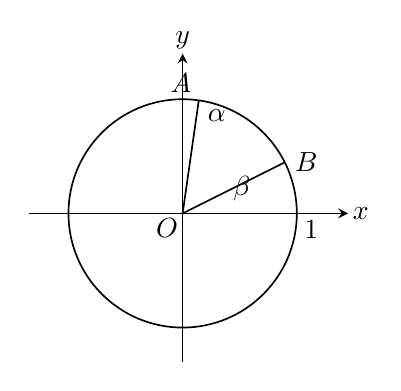
\begin{tikzpicture}[scale=1.45, semithick, every node/.style={inner sep=1.4pt}]
  \draw (0,0) circle [radius=1];
  \draw[->,>=stealth] (-1.35,0) -- (1.45,0) node[right] {$x$};
  \draw[->,>=stealth] (0,-1.3) -- (0,1.4) node[above] {$y$};
  \node[below left] at (0,0) {$O$};

  \coordinate (A) at (0.1414,0.9899);
  \coordinate (B) at (0.8944,0.4472);

  \draw (0,0) -- (A);
  \draw (0,0) -- (B);

  \node[above left=1pt] at (A) {$A$};
  \node[right=2pt] at (B) {$B$};
  \node at (0.30,0.86) {$\alpha$};
  \node at (0.52,0.22) {$\beta$};
  \node[below right=1pt] at (1,0) {$1$};
\end{tikzpicture}
\end{center}
\nopagebreak[4]
\Needspace{4\baselineskip}
\textbf{解析}

\Needspace{5\baselineskip}
（1）由单位圆得 $\cos\alpha=\dfrac{\sqrt2}{10}$，$\sin\alpha=\dfrac{7\sqrt2}{10}$，$\tan\alpha=7$；$\cos\beta=\dfrac{2\sqrt5}5$，$\sin\beta=\dfrac{\sqrt5}5$，$\tan\beta=\dfrac12$。故

\nopagebreak[4]
\[\tan(\alpha+\beta)=\frac{7+\frac12}{1-7\times\frac12}=\frac{15/2}{-5/2}=-3.\]

\Needspace{5\baselineskip}
（2）$\tan2\beta=\dfrac{2\cdot\frac12}{1-\frac14}=\dfrac43$，于是

\nopagebreak[4]
\[\tan(\alpha+2\beta)=\frac{7+\frac43}{1-7\times\frac43}=\frac{25/3}{-25/3}=-1.\]

由 $\alpha$，$\beta$ 为锐角且 $\tan\alpha=7>1$ 知 $\alpha\in\left(\dfrac{\pi}4,\dfrac{\pi}2\right)$，$\tan\beta=\dfrac12<1$ 知 $\beta\in\left(0,\dfrac{\pi}4\right)$，从而 $\alpha+2\beta\in\left(\dfrac{\pi}4,\pi\right)$，故 $\alpha+2\beta=\dfrac{3\pi}4$。

\gkanswer{答案：（1）$-3$；（2）$\dfrac{3\pi}4$。}

\end{answer}
\begin{answer}
\gksolhead{16}{}

\textbf{题目}：

如图，在四面体 $ABCD$ 中，$CB=CD$，$AD\perp BD$，点 $E$、$F$ 分别是 $AB$、$BD$ 的中点。求证：

（1）直线 $EF\parallel$ 平面 $ACD$；

（2）平面 $EFC\perp$ 平面 $BCD$。
\nopagebreak[4]
\begin{center}% 2008 年江苏卷第 16 题：四面体 ABCD，CB=CD，AD⊥BD，E、F 为 AB、BD 中点。
% 来源 PDF：gaokaomath-src/普通高考/2008/2008江苏.pdf
% SHA-256：b998b93963143559a1ce800a6d320de618883b0e22ee5130b7666a2374caeba0
% 原页：2008江苏.pdf 第 1 页（A3 三栏）第 2 栏，书页码 457。
% 绘制依据：按原页斜投影：B 在上、C 在左下、A 在右下、D 在内部（被遮挡）；
%   可见棱 BC、BA、CA 实线，BD、AD、CD 与 EF 虚线，E 在 AB 上、F 在 BD 上。
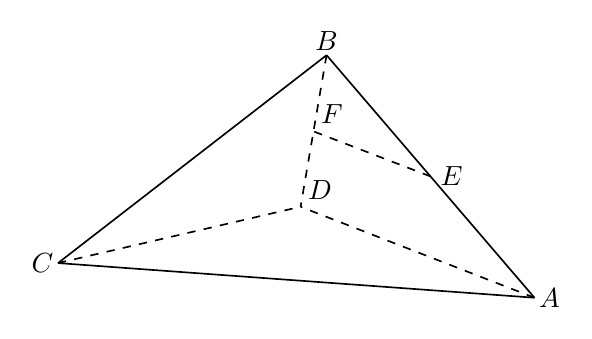
\begin{tikzpicture}[scale=1.1, semithick, every node/.style={inner sep=1.4pt}]
  \coordinate (B) at (3.6,3.3);
  \coordinate (C) at (0.5,0.9);
  \coordinate (A) at (6.0,0.5);
  \coordinate (D) at (3.3,1.55);
  \coordinate (E) at (4.8,1.9);
  \coordinate (F) at (3.45,2.42);

  \draw (B) -- (C);
  \draw (B) -- (A);
  \draw (C) -- (A);

  \draw[dashed] (B) -- (D);
  \draw[dashed] (A) -- (D);
  \draw[dashed] (C) -- (D);
  \draw[dashed] (E) -- (F);

  \node[above] at (B) {$B$};
  \node[left] at (C) {$C$};
  \node[right] at (A) {$A$};
  \node[above right=1pt] at (D) {$D$};
  \node[right=2pt] at (E) {$E$};
  \node[above right=1pt] at (F) {$F$};
\end{tikzpicture}
\end{center}
\nopagebreak[4]
\Needspace{4\baselineskip}
\textbf{解析}

（1）在 $\triangle ABD$ 中，$E$、$F$ 分别为 $AB$、$BD$ 的中点，故 $EF\parallel AD$。又 $AD\subset$ 平面 $ACD$，$EF\not\subset$ 平面 $ACD$，所以 $EF\parallel$ 平面 $ACD$。

（2）由 $CB=CD$ 且 $F$ 为 $BD$ 中点得 $CF\perp BD$；又 $AD\perp BD$ 且 $EF\parallel AD$，故 $EF\perp BD$。于是 $BD\perp$ 平面 $EFC$，而 $BD\subset$ 平面 $BCD$，所以平面 $EFC\perp$ 平面 $BCD$。

\gkanswer{答案：（1）（2）证明见解析。}

\end{answer}
\begin{answer}
\gksolhead{17}{}

\textbf{题目}：

如图，某地有三家工厂，分别位于矩形 $ABCD$ 的两个顶点 $A$、$B$ 及 $CD$ 的中点 $P$ 处，已知 $AB=20$ km，$BC=10$ km。为了处理三家工厂的污水，现要在矩形区域上（含边界），且与 $A$、$B$ 等距离的一点 $O$ 处建造一个污水处理厂，并铺设三条排污管道 $AO$、$BO$、$PO$。记排污管道的总长度为 $y$ km。

（1）按下列要求写出函数关系式：

① 设 $\angle BAO=\theta$（rad），将 $y$ 表示为 $\theta$ 的函数；

② 设 $OP=x$（km），将 $y$ 表示为 $x$ 的函数；

（2）请你选用（1）中的一个函数关系式，确定污水处理厂的位置，使铺设的排污管道的总长度最短。
\nopagebreak[4]
\begin{center}% 2008 年江苏卷第 17 题：矩形厂区 ABCD，工厂在 A、B 与 CD 中点 P，污水处理厂在 O。
% 来源 PDF：gaokaomath-src/普通高考/2008/2008江苏.pdf
% SHA-256：b998b93963143559a1ce800a6d320de618883b0e22ee5130b7666a2374caeba0
% 原页：2008江苏.pdf 第 1 页（A3 三栏）第 3 栏，书页码 457。
% 绘制依据：按原页画矩形 ABCD（AB 在下、CD 在上），P 在 CD 中点，O 在矩形内部
%   且在 AB 的垂直平分线上，连 OA、OB、OP。
\begin{tikzpicture}[scale=0.62, semithick, every node/.style={inner sep=1.4pt}]
  \draw (0,0) rectangle (20,10);
  \coordinate (A) at (0,0);
  \coordinate (B) at (20,0);
  \coordinate (C) at (20,10);
  \coordinate (D) at (0,10);
  \coordinate (P) at (10,10);
  \coordinate (O) at (10,5.8);

  \draw (O) -- (A);
  \draw (O) -- (B);
  \draw (O) -- (P);

  \node[below left] at (A) {$A$};
  \node[below right] at (B) {$B$};
  \node[above right] at (C) {$C$};
  \node[above left] at (D) {$D$};
  \node[above] at (P) {$P$};
  \node[right=1pt] at (O) {$O$};
\end{tikzpicture}
\end{center}
\nopagebreak[4]
\Needspace{4\baselineskip}
\textbf{解析}

\Needspace{5\baselineskip}
（1）① 设 $O$ 到 $AB$ 的距离为 $h$，则 $h=10\tan\theta$，$OA=OB=\dfrac{10}{\cos\theta}$，$PO=10-h$，故

\nopagebreak[4]
\[y=\frac{20}{\cos\theta}+10-10\tan\theta.\]

\Needspace{5\baselineskip}
② $OP=x$ 时 $h=10-x$，$OA=OB=\sqrt{100+(10-x)^2}$，故

\nopagebreak[4]
\[y=2\sqrt{100+(10-x)^2}+x.\]

\Needspace{5\baselineskip}
（2）用②，令 $t=10-x\in[0,10]$，则 $y=2\sqrt{100+t^2}+10-t$，

\nopagebreak[4]
\[y'=\frac{2t}{\sqrt{100+t^2}}-1=0\iff t=\frac{10}{\sqrt3},\]

\Needspace{5\baselineskip}
且 $y'$ 在 $\left(0,\frac{10}{\sqrt3}\right)$ 上为负、在 $\left(\frac{10}{\sqrt3},10\right)$ 上为正，故最小值

\nopagebreak[4]
\[y_{\min}=2\cdot\frac{20}{\sqrt3}+10-\frac{10}{\sqrt3}=10+10\sqrt3.\]

\gkanswer{答案：（1）① $y=\dfrac{20}{\cos\theta}-10\tan\theta+10$（$0\leqslant\theta\leqslant\frac{\pi}4$）；② $y=2\sqrt{100+(10-x)^2}+x$（$0\leqslant x\leqslant10$）；（2）$OA=OB=PB=PA$ 即 $O$ 在 $AB$ 中垂线上距 $AB$ $\dfrac{10\sqrt3}3$ km 处，最短总长度 $\left(10+10\sqrt3\right)$ km。}

\end{answer}
\begin{answer}
\gksolhead{18}{}

\textbf{题目}：

在平面直角坐标系 $xOy$ 中，设二次函数 $f(x)=x^2+2x+b$（$x\in\mathbf R$）的图象与两坐标轴有三个交点，经过这三个交点的圆记为 $C$。

（1）求实数 $b$ 的取值范围；

（2）求圆 $C$ 的方程；

（3）问圆 $C$ 是否经过定点（其坐标与 $b$ 无关）？请证明你的结论。

\Needspace{4\baselineskip}
\textbf{解析}

（1）图象与两坐标轴有三个交点，需与 $x$ 轴有两个不同交点且都不过原点：$\Delta=4-4b>0$ 且 $b\neq0$，即 $b<1$ 且 $b\neq0$。

\Needspace{5\baselineskip}
（2）设 $x$ 轴两交点横坐标为 $x_1$、$x_2$，则 $x_1+x_2=-2$，$x_1x_2=b$；$y$ 轴交点为 $(0,b)$。设圆 $x^2+y^2+Dx+Ey+F=0$，由 $x^2+Dx+F=0$ 的两根为 $x_1$、$x_2$ 得 $D=2$，$F=b$；代入 $(0,b)$ 得 $b^2+Eb+b=0$，即 $E=-(b+1)$。故

\nopagebreak[4]
\[x^2+y^2+2x-(b+1)y+b=0.\]

（3）方程整理为 $(x^2+y^2+2x-y)+b(1-y)=0$。令 $1-y=0$ 且 $x^2+y^2+2x-y=0$，得 $y=1$，$x^2+2x=0$，即 $x=0$ 或 $x=-2$。故圆 $C$ 恒过定点 $(0,1)$ 与 $(-2,1)$。

\gkanswer{答案：（1）$b<1$ 且 $b\neq0$；（2）$x^2+y^2+2x-(b+1)y+b=0$；（3）过定点 $(0,1)$ 与 $(-2,1)$。}

\end{answer}
\begin{answer}
\gksolhead{19}{}

\textbf{题目}：

（1）设 $a_1$，$a_2$，$\cdots$，$a_n$ 是各项均不为零的 $n$（$n\geqslant4$）项等差数列，且公差 $d\neq0$。若将此数列删去某一项得到的数列（按原来的顺序）是等比数列，

① 当 $n=4$ 时，求 $\dfrac{a_1}d$ 的数值；

② 求 $n$ 的所有可能值。

（2）求证：对于给定的正整数 $n$（$n\geqslant4$），存在一个各项及公差都不为零的等差数列 $b_1$，$b_2$，$\cdots$，$b_n$，其中任意三项（按原来顺序）都不能组成等比数列。

\Needspace{4\baselineskip}
\textbf{解析}

（1）① $n=4$ 时删去一项得三项。删 $a_2$：$a_1,a_3,a_4$ 成等比，$(a+2d)^2=a(a+3d)$，得 $a=-4d$，$\dfrac{a_1}d=-4$；删 $a_3$：$a_1,a_2,a_4$ 成等比，$(a+d)^2=a(a+3d)$，得 $a=d$，$\dfrac{a_1}d=1$；删 $a_1$ 或 $a_4$ 时由等比条件均得 $d=0$，不合。故 $\dfrac{a_1}d=-4$ 或 $1$。

② 若删去的项不在首尾三项之内，则余下数列的前三项或后三项仍是 $a$、$a+d$、$a+2d$ 型，成等比必推出 $d=0$，矛盾；逐项检验可知只有 $n=4$ 可行（$n=5$ 时删中间项的要求互相矛盾）。故 $n=4$。

\Needspace{5\baselineskip}
（2）取 $b_k=a+(k-1)d$（$d\neq0$，$a\neq0$）。若某三项 $b_i,b_j,b_l$（$i<j<l$）成等比，则

\nopagebreak[4]
\[(a+(j-1)d)^2=(a+(i-1)d)(a+(l-1)d),\]

展开消去 $a^2$ 得 $a(2j-i-l)=d\left[(i-1)(l-1)-(j-1)^2\right]$。

当 $2j-i-l=0$ 时，右端为 $d(il-j^2)$，由 $i<l$ 知 $il<j^2$，故右端非零，等式不成立；当 $2j-i-l\neq0$ 时，$a$ 至多取一个被禁止的值。三项组合只有有限多个，故只有有限多个 $a$ 值使某三项成等比，取其余任一非零 $a$ 即可。

\gkanswer{答案：（1）① $-4$ 或 $1$；② $n=4$；（2）证明见解析。}

\end{answer}
\begin{answer}
\gksolhead{20}{}

\textbf{题目}：

已知函数 $f_1(x)=3^{|x-p_1|}$，$f_2(x)=2\cdot3^{|x-p_2|}$（$x\in\mathbf R$，$p_1$，$p_2$ 为常数）。函数 $f(x)$ 定义为：对每个给定的实数 $x$，$f(x)=\begin{cases}f_1(x),&\text{\text{若} }f_1(x)\leqslant f_2(x),\\f_2(x),&\text{\text{若} }f_1(x)>f_2(x).\end{cases}$

（1）求 $f(x)=f_1(x)$ 对所有实数 $x$ 成立的充分必要条件（用 $p_1$，$p_2$ 表示）；

（2）设 $a$，$b$ 是两个实数，满足 $a<b$，且 $p_1$，$p_2\in(a,b)$。若 $f(a)=f(b)$，求证：$f(x)$ 在区间 $[a,b]$ 上的单调增区间的长度之和为 $\dfrac{b-a}2$。（闭区间 $[m,n]$ 的长度定义为 $n-m$）

\Needspace{4\baselineskip}
\textbf{解析}

\Needspace{5\baselineskip}
（1）$f(x)=f_1(x)$ 恒成立等价于 $f_1(x)\leqslant f_2(x)$ 恒成立，即

\nopagebreak[4]
\[3^{|x-p_1|-|x-p_2|}\leqslant2\iff|x-p_1|-|x-p_2|\leqslant\log_32.\]

由三角不等式，$|x-p_1|-|x-p_2|$ 的最大值为 $|p_1-p_2|$，故充要条件为 $|p_1-p_2|\leqslant\log_32$。

（2）不妨设 $p_1<p_2$，记 $d=p_2-p_1$。函数 $h(x)=|x-p_1|-|x-p_2|$ 在 $x\leqslant p_1$ 时为 $-d$，在 $[p_1,p_2]$ 上线性递增到 $d$，在 $x\geqslant p_2$ 时为 $d$；又 $f=f_1\iff h\leqslant\log_32$。

若 $d\leqslant\log_32$，则 $f=f_1$ 恒成立，由 $f(a)=f(b)$ 得 $p_1-a=b-p_1$，即 $p_1=\dfrac{a+b}2$，此时 $f$ 在 $[a,p_1]$ 递减、$[p_1,b]$ 递增，增区间长度为 $b-p_1=\dfrac{b-a}2$。

若 $d>\log_32$，设 $x_0\in(p_1,p_2)$ 满足 $h(x_0)=\log_32$。则 $f=f_1$ 于 $[a,x_0]$、$f=f_2$ 于 $[x_0,b]$，故 $f$ 的增区间为 $[p_1,x_0]$ 与 $[p_2,b]$，长度之和为 $(x_0-p_1)+(b-p_2)$。

\Needspace{5\baselineskip}
由 $f(a)=f(b)$，即 $3^{p_1-a}=2\cdot3^{b-p_2}$，取对数得 $p_1-a=b-p_2+\log_32$，而 $x_0=\dfrac{p_1+p_2+\log_32}2$，代入得

\nopagebreak[4]
\[(x_0-p_1)+(b-p_2)=\frac{p_2-p_1+\log_32}2+(b-p_2)=\frac{b-a}2.\]

两种情形下增区间长度之和均为 $\dfrac{b-a}2$。

\gkanswer{答案：（1）$|p_1-p_2|\leqslant\log_32$；（2）证明见解析。}

\end{answer}
\begin{answer}
\gksolhead{21}{}

\textbf{题目}：

四选二。

【A】如图，设 $\triangle ABC$ 的外接圆的切线 $AE$ 与 $BC$ 的延长线交于点 $E$，$\angle BAC$ 的平分线与 $BC$ 交于点 $D$。求证：$ED^2=EC\cdot EB$。
\nopagebreak[4]
\begin{center}% 2008 年江苏卷第 21A 题：△ABC 的外接圆，切线 AE 与 BC 延长线交于 E，AD 平分 ∠BAC。
% 来源 PDF：gaokaomath-src/普通高考/2008/2008江苏.pdf
% SHA-256：b998b93963143559a1ce800a6d320de618883b0e22ee5130b7666a2374caeba0
% 原页：2008江苏.pdf 第 2 页（A3 三栏）第 2 栏，书页码 458。
% 绘制依据：按原页画圆、圆上 A（上）、B（左上）、C（右下），BC 延长线上的 E，
%   切线 AE，以及 ∠BAC 的平分线 AD（D 在 BC 上）。
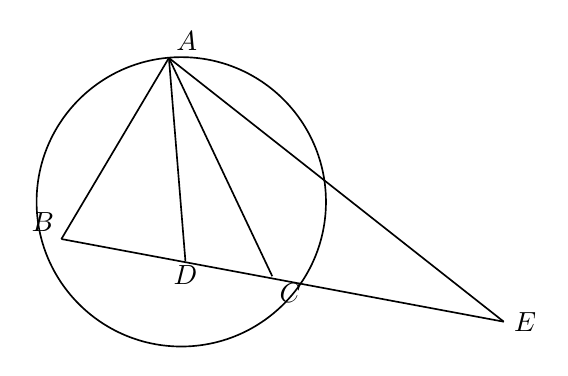
\begin{tikzpicture}[scale=1.05, semithick, every node/.style={inner sep=1.4pt}]
  % 外接圆
  \draw (2.2,1.5) circle [radius=1.75];

  \coordinate (A) at (2.05,3.24);
  \coordinate (B) at (0.75,1.05);
  \coordinate (C) at (3.30,0.60);
  \coordinate (D) at (2.25,0.78);
  \coordinate (E) at (6.10,0.05);

  \draw (B) -- (E);
  \draw (A) -- (B);
  \draw (A) -- (C);
  \draw (A) -- (E);
  \draw (A) -- (D);

  \node[above right=1pt] at (A) {$A$};
  \node[above left=1pt] at (B) {$B$};
  \node[below right=1pt] at (C) {$C$};
  \node[below] at (D) {$D$};
  \node[right=2pt] at (E) {$E$};
\end{tikzpicture}
\end{center}
\nopagebreak[4]
【B】在平面直角坐标系 $xOy$ 中，设椭圆 $4x^2+y^2=1$ 在矩阵 $\boldsymbol A=\begin{bmatrix}2&0\\0&1\end{bmatrix}$ 对应的变换下得到曲线 $F$，求 $F$ 的方程。

【C】在平面直角坐标系 $xOy$ 中，设 $P(x,y)$ 是椭圆 $\dfrac{x^2}3+y^2=1$ 上的一个动点，求 $S=x+y$ 的最大值。

【D】设 $a$，$b$，$c$ 为正实数，求证：$\dfrac1{a^3}+\dfrac1{b^3}+\dfrac1{c^3}+abc\geqslant2\sqrt3$。

\Needspace{4\baselineskip}
\textbf{解析}

\Needspace{5\baselineskip}
【A】由切割线定理 $EA^2=EC\cdot EB$，故只需证 $ED=EA$。由 $AE$ 为切线得 $\angle EAC=\angle ABC$（弦切角），又 $AD$ 平分 $\angle BAC$，故

\nopagebreak[4]
\[\angle EAD=\angle EAC+\angle CAD=\angle ABC+\angle BAD,\]

而 $\angle EDA$ 是 $\triangle ABD$ 的外角，$\angle EDA=\angle ABD+\angle BAD$。两式相等，故 $EA=ED$，从而 $ED^2=EC\cdot EB$。

【B】设变换后曲线上点为 $(x',y')$，则 $x'=2x$，$y'=y$，即 $x=\dfrac{x'}2$，$y=y'$。代入 $4x^2+y^2=1$ 得 $x'^2+y'^2=1$，故 $F$ 的方程为 $x^2+y^2=1$。

\Needspace{5\baselineskip}
【C】令 $x=\sqrt3\cos\theta$，$y=\sin\theta$，则

\nopagebreak[4]
\[S=\sqrt3\cos\theta+\sin\theta=2\sin\left(\theta+\frac{\pi}3\right)\leqslant2,\]

最大值为 $2$。

\Needspace{5\baselineskip}
【D】由均值不等式 $\dfrac1{a^3}+\dfrac1{b^3}+\dfrac1{c^3}\geqslant\dfrac3{abc}$，故

\nopagebreak[4]
\[\frac1{a^3}+\frac1{b^3}+\frac1{c^3}+abc\geqslant\frac3{abc}+abc\geqslant2\sqrt3,\]

当 $a=b=c=1$ 时取等号。

\gkanswer{答案：A 证明见解析；B $x^2+y^2=1$；C $2$；D 证明见解析。}

\end{answer}
\begin{answer}
\gksolhead{22}{}

\textbf{题目}：

如图，设动点 $P$ 在棱长为 $1$ 的正方体 $ABCD-A_1B_1C_1D_1$ 的对角线 $BD_1$ 上，记 $\dfrac{D_1P}{D_1B}=\lambda$。当 $\angle APC$ 为钝角时，求 $\lambda$ 的取值范围。
\nopagebreak[4]
\begin{center}% 2008 年江苏卷第 22 题：棱长 1 的正方体，P 在对角线 BD1 上。
% 来源 PDF：gaokaomath-src/普通高考/2008/2008江苏.pdf
% SHA-256：b998b93963143559a1ce800a6d320de618883b0e22ee5130b7666a2374caeba0
% 原页：2008江苏.pdf 第 2 页（A3 三栏）第 3 栏，书页码 458。
% 绘制依据：按原页斜投影：上底 A1B1C1D1、下底 ABCD，P 在 BD1 上；
%   被遮挡的棱 A1D1、D1C1、DD1 与 BD1、AP、CP 用虚线。
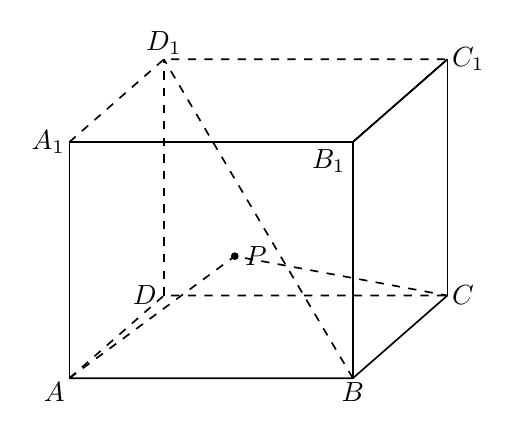
\begin{tikzpicture}[scale=1.0, semithick, every node/.style={inner sep=1.4pt}]
  \coordinate (A) at (0.00,0.00);
  \coordinate (B) at (3.60,0.00);
  \coordinate (C) at (4.80,1.05);
  \coordinate (D) at (1.20,1.05);
  \coordinate (A1) at (0.00,3.00);
  \coordinate (B1) at (3.60,3.00);
  \coordinate (C1) at (4.80,4.05);
  \coordinate (D1) at (1.20,4.05);
  \coordinate (P) at (2.10,1.55);

  \draw (A) -- (B) -- (C);
  \draw (A) -- (A1);
  \draw (B) -- (B1);
  \draw (C) -- (C1);
  \draw (A1) -- (B1) -- (C1);
  \draw (B1) -- (C1);

  \draw[dashed] (A) -- (D) -- (C);
  \draw[dashed] (D) -- (D1);
  \draw[dashed] (A1) -- (D1) -- (C1);
  \draw[dashed] (B) -- (D1);
  \draw[dashed] (A) -- (P) -- (C);

  \fill (P) circle (1.4pt);

  \node[below left] at (A) {$A$};
  \node[below] at (B) {$B$};
  \node[right] at (C) {$C$};
  \node[left=1pt] at (D) {$D$};
  \node[left] at (A1) {$A_1$};
  \node[below left=1pt] at (B1) {$B_1$};
  \node[right] at (C1) {$C_1$};
  \node[above] at (D1) {$D_1$};
  \node[right=2pt] at (P) {$P$};
\end{tikzpicture}
\end{center}
\nopagebreak[4]
\Needspace{4\baselineskip}
\textbf{解析}

\Needspace{5\baselineskip}
以 $A$ 为原点，$AB$、$AD$、$AA_1$ 为 $x$、$y$、$z$ 轴，则 $B(1,0,0)$，$C(1,1,0)$，$D_1(0,1,1)$。由 $\overrightarrow{D_1P}=\lambda\overrightarrow{D_1B}$ 得

\nopagebreak[4]
\[P=(\lambda,\,1-\lambda,\,1-\lambda).\]

\Needspace{5\baselineskip}
于是

\nopagebreak[4]
\[\overrightarrow{PA}=(-\lambda,\lambda-1,\lambda-1),\qquad \overrightarrow{PC}=(1-\lambda,\lambda,\lambda-1),\]

\nopagebreak[4]
\[\overrightarrow{PA}\cdot\overrightarrow{PC}=3\lambda^2-4\lambda+1=(3\lambda-1)(\lambda-1).\]

$\angle APC$ 为钝角需该式小于 $0$，即 $\dfrac13<\lambda<1$。

\gkanswer{答案：$\lambda\in\left(\dfrac13,1\right)$。}

\end{answer}
\begin{answer}
\gksolhead{23}{}

\textbf{题目}：

请先阅读：在等式 $\cos2x=2\cos^2x-1$（$x\in\mathbf R$）的两边对 $x$ 求导：$(\cos2x)'=(2\cos^2x-1)'$。由求导法则得 $(-\sin2x)\cdot2=4\cos x\cdot(-\sin x)$，化简得等式 $\sin2x=2\sin x\cos x$。

（1）利用上述想法（或者其他方法），试由等式 $(1+x)^n=\mathrm C_n^0+\mathrm C_n^1x+\mathrm C_n^2x^2+\cdots+\mathrm C_n^nx^n$（$x\in\mathbf R$，整数 $n\geqslant2$）证明：$n\left[(1+x)^{n-1}-1\right]=\sum\limits_{k=2}^nk\mathrm C_n^kx^{k-1}$；

（2）对于正整数 $n\geqslant3$，求证：

① $\sum\limits_{k=1}^n(-1)^kk\mathrm C_n^k=0$；

② $\sum\limits_{k=1}^n(-1)^kk^2\mathrm C_n^k=0$；

③ $\sum\limits_{k=0}^n\dfrac1{k+1}\mathrm C_n^k=\dfrac{2^{n+1}-1}{n+1}$。

\Needspace{4\baselineskip}
\textbf{解析}

\Needspace{5\baselineskip}
（1）对 $(1+x)^n=\sum\limits_{k=0}^n\mathrm C_n^kx^k$ 两边求导：

\nopagebreak[4]
\[n(1+x)^{n-1}=\sum_{k=1}^nk\mathrm C_n^kx^{k-1}.\]

\Needspace{5\baselineskip}
两端同减 $n$（即 $k=1$ 的那一项 $\mathrm C_n^1x^0=n$）得

\nopagebreak[4]
\[n\left[(1+x)^{n-1}-1\right]=\sum_{k=2}^nk\mathrm C_n^kx^{k-1}.\]

\Needspace{5\baselineskip}
（2）① 在（1）的等式中令 $x=-1$（$n\geqslant3$ 时左端为 $-n$）：

\nopagebreak[4]
\[-n=\sum_{k=2}^nk\mathrm C_n^k(-1)^{k-1}\iff\sum_{k=2}^n(-1)^kk\mathrm C_n^k=n,\]

故 $\sum\limits_{k=1}^n(-1)^kk\mathrm C_n^k=-n+n=0$。

\Needspace{5\baselineskip}
② 把（1）中的等式两端乘以 $x$ 再求导：

\nopagebreak[4]
\[n\left[(1+x)^{n-1}+(n-1)x(1+x)^{n-2}\right]=\sum_{k=1}^nk^2\mathrm C_n^kx^{k-1}.\]

\Needspace{5\baselineskip}
令 $x=-1$，右端为 $\sum k^2\mathrm C_n^k(-1)^{k-1}$，左端两项均含因子 $(1+x)$ 的幂（$n\geqslant3$ 时取值为 $0$），故

\nopagebreak[4]
\[\sum_{k=1}^n(-1)^kk^2\mathrm C_n^k=0.\]

\Needspace{5\baselineskip}
③ 由 $\dfrac1{k+1}\mathrm C_n^k=\dfrac1{n+1}\mathrm C_{n+1}^{k+1}$，

\nopagebreak[4]
\[\sum_{k=0}^n\frac1{k+1}\mathrm C_n^k=\frac1{n+1}\sum_{k=0}^n\mathrm C_{n+1}^{k+1}=\frac1{n+1}\left(2^{n+1}-1\right).\]

\gkanswer{答案：（1）（2）证明见解析。}

\end{answer}